\section{方法描述}
\label{sec:5_method}

对于一个标准的图片信息辅助式神经机器翻译,其输入为一个源语言句子$X$和一个与其对应的图片$I$,然后利用这两个模态的信息生成翻译$Y$。然而,现有的很多方法对输入图片$I$中的信息并不敏感。这是因为翻译任务所使用的数据中,大部分$X$与$Y$之间有着很好的语义对齐关系。这使得翻译模型在不依靠图片输入的情况下,就可以在训练阶段学习到一组相对不错的模型参数,使模型很容易收敛到一个不需要图片信息的局部最优解。为了使机器翻译模型充分利用为句子提供的图片信息,本章提出了基于图文对比对抗训练的神经机器翻译方法。本节将首先介绍本章所使用的翻译模型结构,然后详细介绍如何通过对比对抗训练增加模型对视觉信息的敏感度。

\subsection{模型结构}
\label{sec:5_architecture}
\begin{figure}[!htbp]
    \centering
    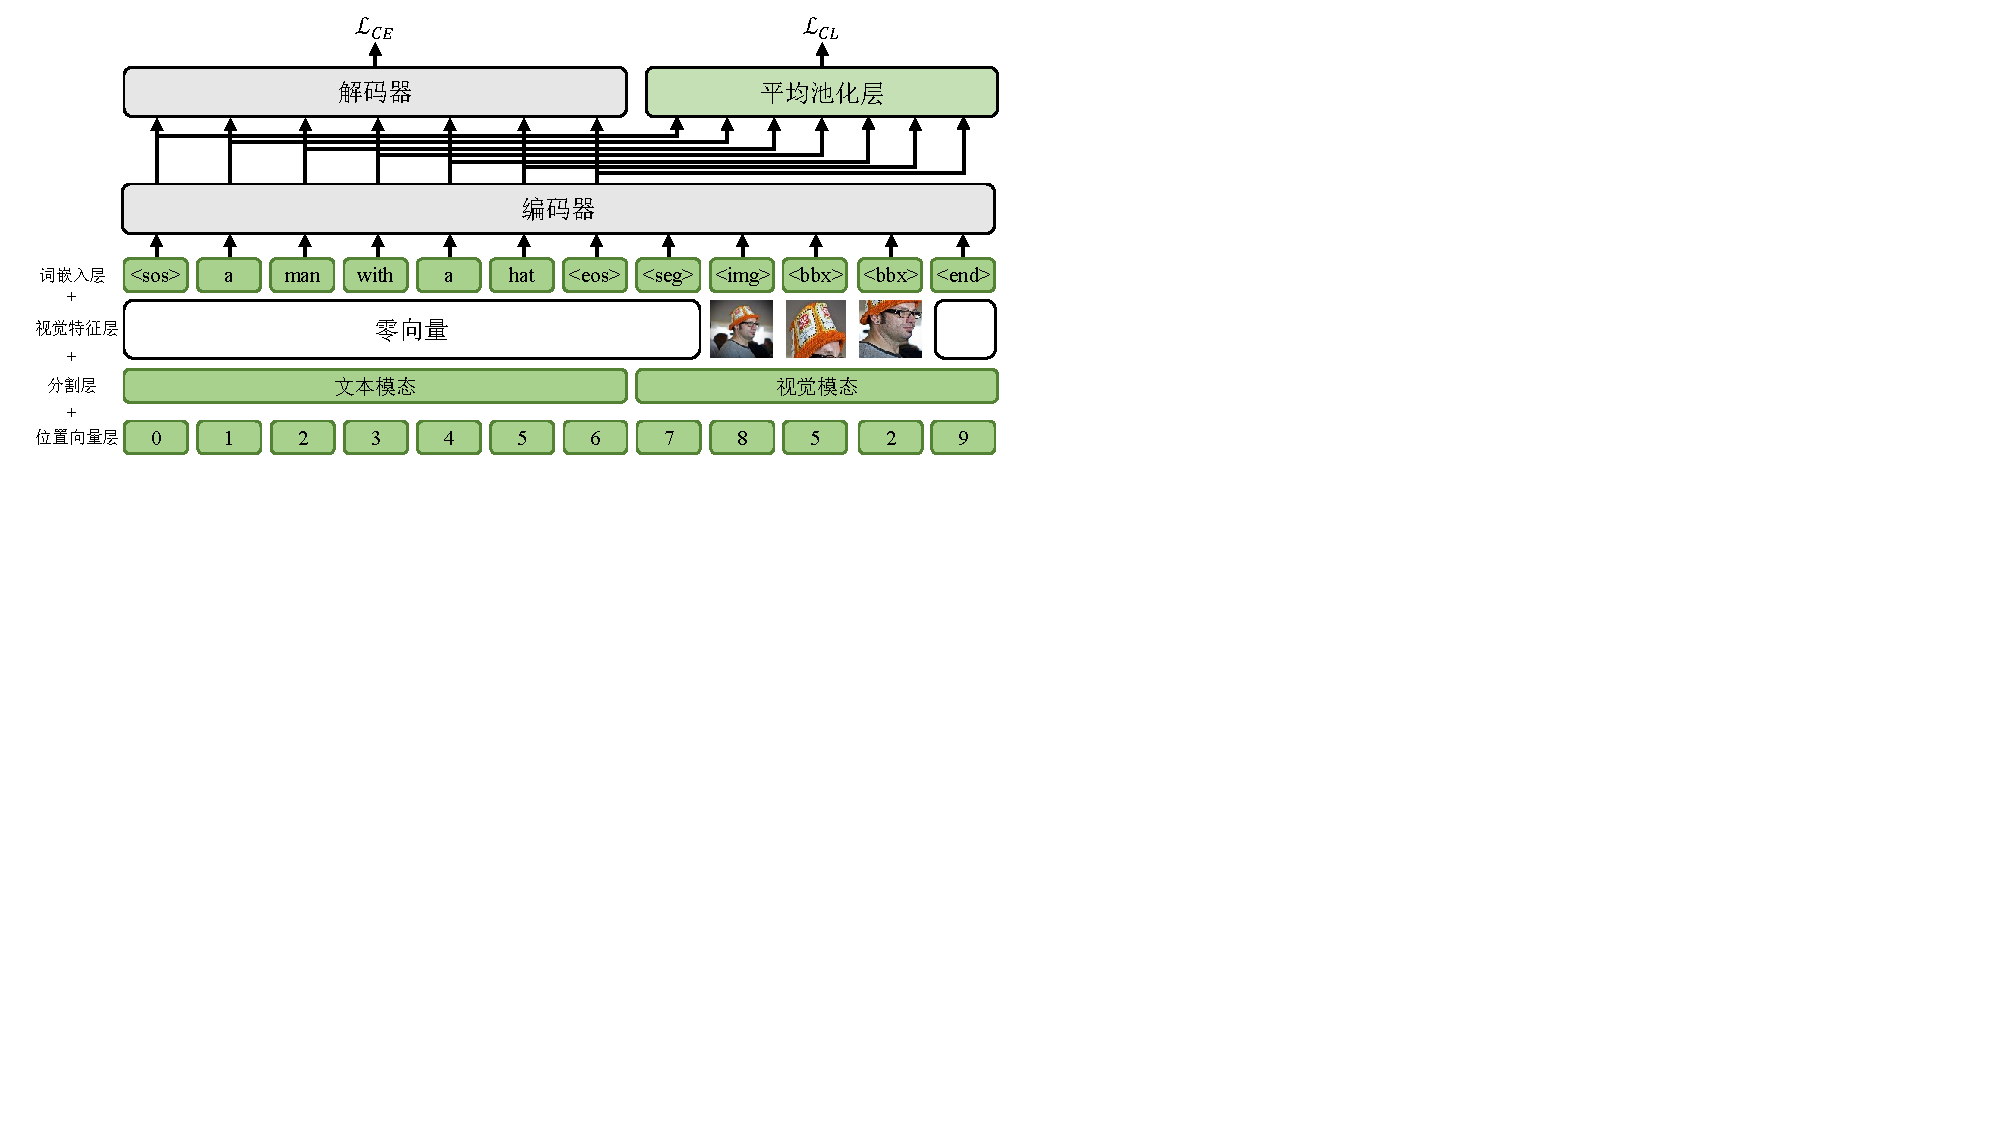
\includegraphics[scale=0.85]{Img/fig_5_model.pdf}
    \bicaption{结合对比对抗训练方法的神经机器翻译模型}{NMT model combined with contrastive adversarial training method}
    \label{fig:5_model}
\end{figure}
本章采用了一种句子级跨模态语义融合模型结构,其输入为一个文本序列,和一个可选的视觉输入,该视觉输入为文本序列对应的完整图片以及图片内部的数个视觉目标,如图\ref{fig:5_model}所示。该模型的编码器和解码器为常规的Transformer结构。其中,Transformer的编码器负责跨模态信息融合。为了使Transformer支持文本加图片形式的输入,本文采用了一个跨模态嵌入层。该嵌入层共分为4个子层:词嵌入层,视觉特征层,模态分割层,位置编码层。

(1){\sffamily 词嵌入层:}为了支持图片的输入,需要在词嵌入层对应的词表中,加入一些特殊字符:“<seg>”将词嵌入层输入的前后两部分分割为文本和视觉两个序列;“<img>”代表着放置完整图片的位置,每个输入序列仅一个;“<bbx>”代表放置图片中的视觉目标的位置,每个输入序列可以有多个;“<end>”代表着跨模态输入序列的结尾。


(2){\sffamily 视觉特征层:}该层每个位置的输入与词嵌入层的特殊字符相对应,其中“<img>”的对应位置放置输入的完整图片的全局特征,“<bbx>”对应位置放置视觉目标的全局特征,其它位置输入零向量。


(3){\sffamily 分割层:}这一层的作用相对简单,主要用作标识每个位置的输入属于文本序列还是图片序列。因此一共只有“文本模态”和“视觉模态”两个值,每个值都是与词嵌入层维度相同的向量。其中“<seg>”之前的文本序列均对应着“文本模态”,“<seg>”以及其后面的序列均为“视觉模态”。


(4){\sffamily 位置向量层:}这一层与一般的位置向量作用相似,能够表示输入序列中的绝对位置关系。区别在于,当输入的视觉目标与文本中的某些词有对应关系时,可以将视觉目标的位置设置为与其对应的词相同的位置,从而达到加强图片信息作用准确性的目的。如图\ref{fig:5_model}所示,图片输入序列中的“帽子”的绝对位置为5,与文本序列中的“hat”保持一致。

在解码阶段,解码器仅接收“文本模态”的编码结果作为输入。这是因为本章的CAT方法旨在帮助神经机器翻译模型将视觉信息融合到文本表示中。而该过程发生在编码阶段,即没有针对解码器采取翻译以外的优化方法。因此,基于常规的神经机器翻译模型对视觉信息不敏感的假设,其内部模块,如解码器,往往也会忽略视觉信息的输入。所以,将“视觉模态”部分的隐层单元传递给解码器是多余的。

图\ref{fig:5_model}中可以看到,CAT-NMT的目标函数包含了两个部分:融合图片信息的神经机器翻译所需的交叉熵(cross entropy,CE)损失函数和CAT所需的对比损失函数。其中交叉熵损失函数为:
\begin{equation}
    \mathcal{L}_{CE}(\phi, \theta, \psi)=-\sum_j^M \log p(y_j|y_{<j},X,I)
\label{eq:5_cross_entropy}
\end{equation}
其中,$y_j \in Y,j=1,\cdots,M$,$\phi$为解码器参数,$\theta$为编码器参数,$\psi$为跨模态嵌入层的参数。该损失函数与常规的图片信息辅助式神经机器翻译模型相似,均是通过源语言句子$X$和对应图片$I$为输入信息,生成翻译$Y$的形式。在本章的方案中,$I$代表了完整的图片信息,在模型输入中表示为完整图片和其中的多个视觉目标的组合。该损失函数无法反映出的信息是,本章的跨模态信息融合过程,仅发生在编码端。图\ref{fig:5_model}中除了平均池化(average pooling)层,其它参数均需要通过翻译任务来优化。

\subsection{对比对抗训练}
\label{sec:5_cat}
正如上一节介绍,本章是在Transformer的编码器中实现将图片信息或视觉目标信息融合到文本的表示中。然而,基于常规的神经机器翻译模型对视觉信息不敏感的假设,在没有额外的引导下,编码器同样会忽略图片信息的存在。为了有效地融合视觉信息,本章提出了图文对比对抗方法实现在编码过程将图片信息融合到文本的表示中。CAT方法主要包含三部分:对比学习,对抗训练以及双向翻译训练。

\begin{figure}[H]
    \centering
    \begin{subfigure}[b]{0.3\textwidth} % default 0.25\textwidth
    %\begin{minipage}[t]{0.33\linewidth}
      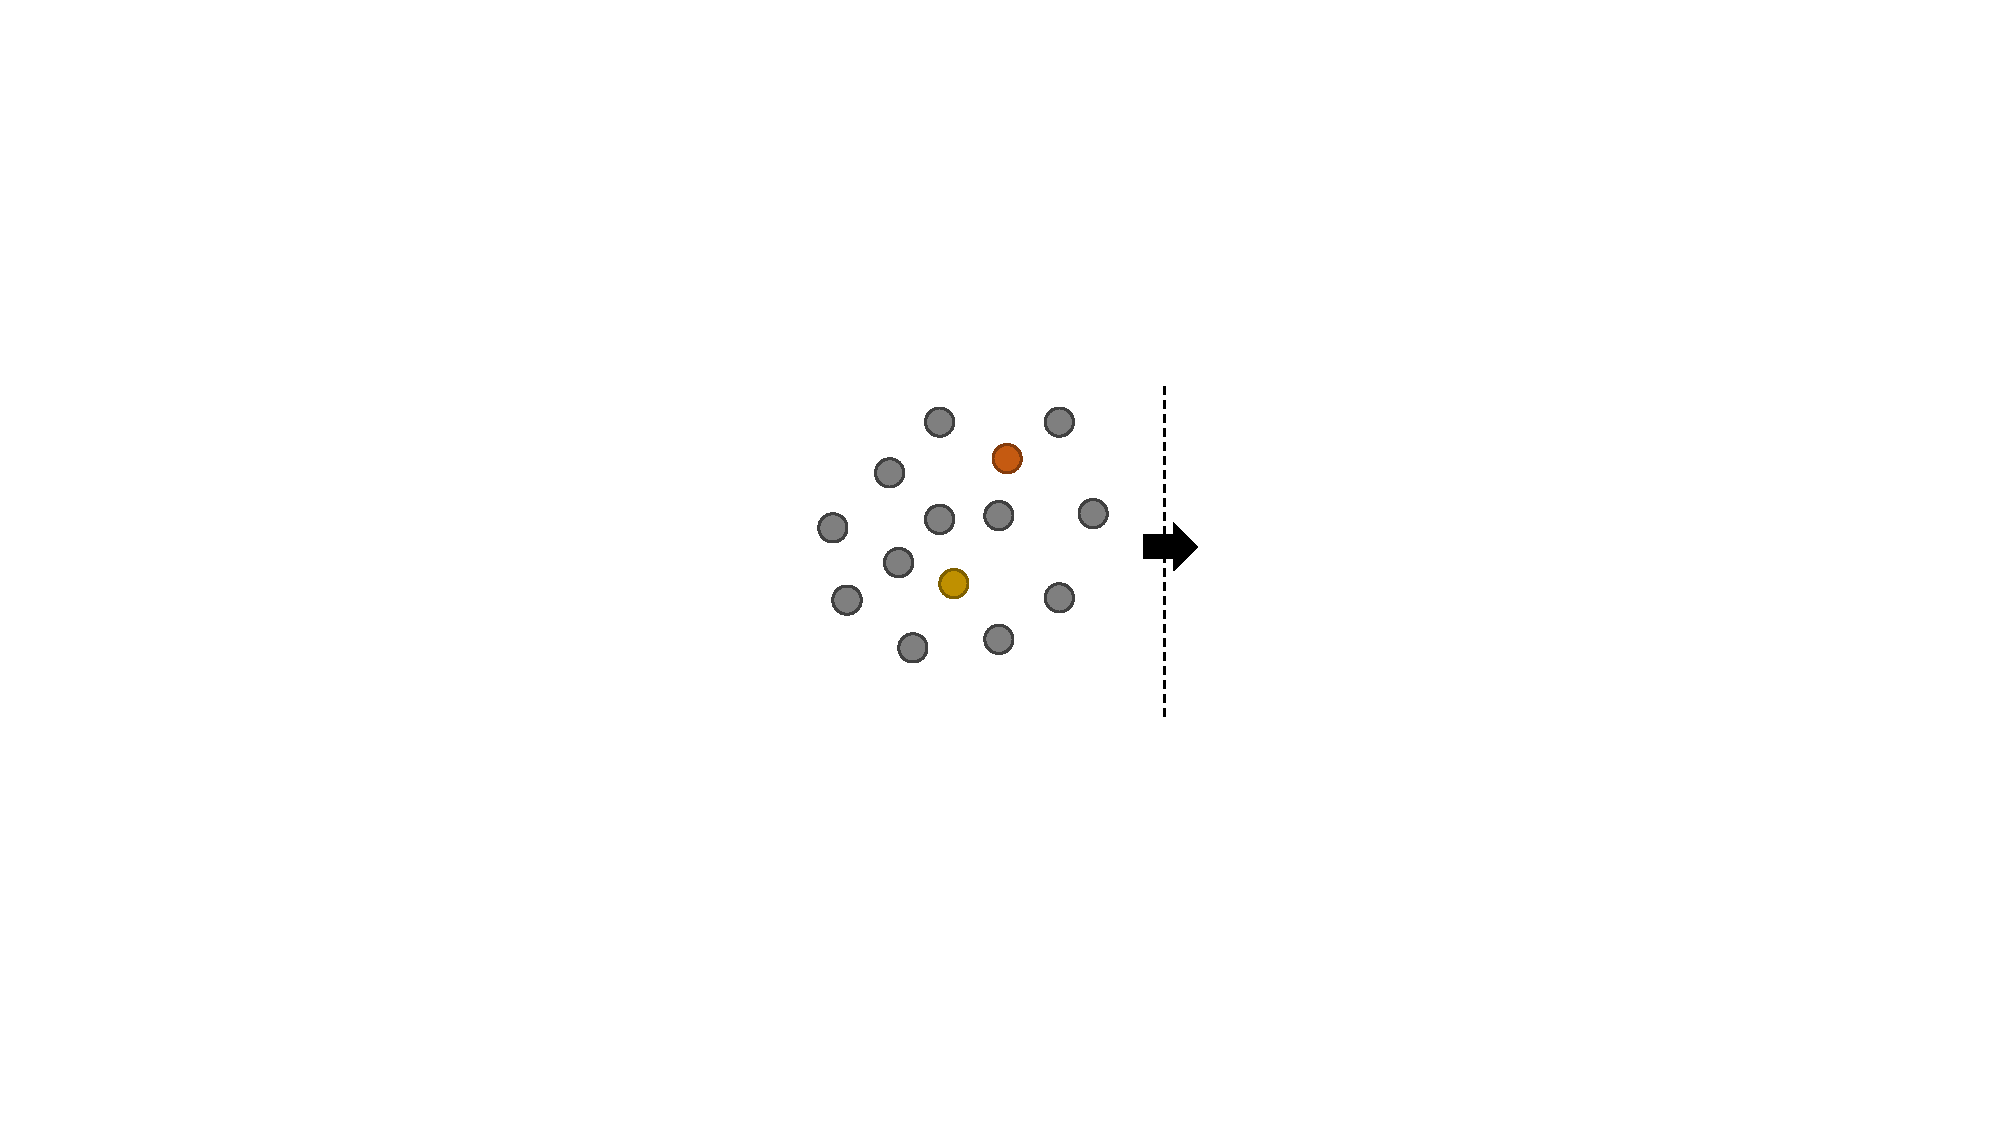
\includegraphics[width=\textwidth]{Img/fig_5_cat_a.pdf}
      \caption{}
      \label{fig:5_cat_a}
    %\end{minipage}
    \end{subfigure}%
    ~% add desired spacing
    \begin{subfigure}[b]{0.26\textwidth} % default 0.23\textwidth
    %\begin{minipage}[t]{0.33\linewidth}
      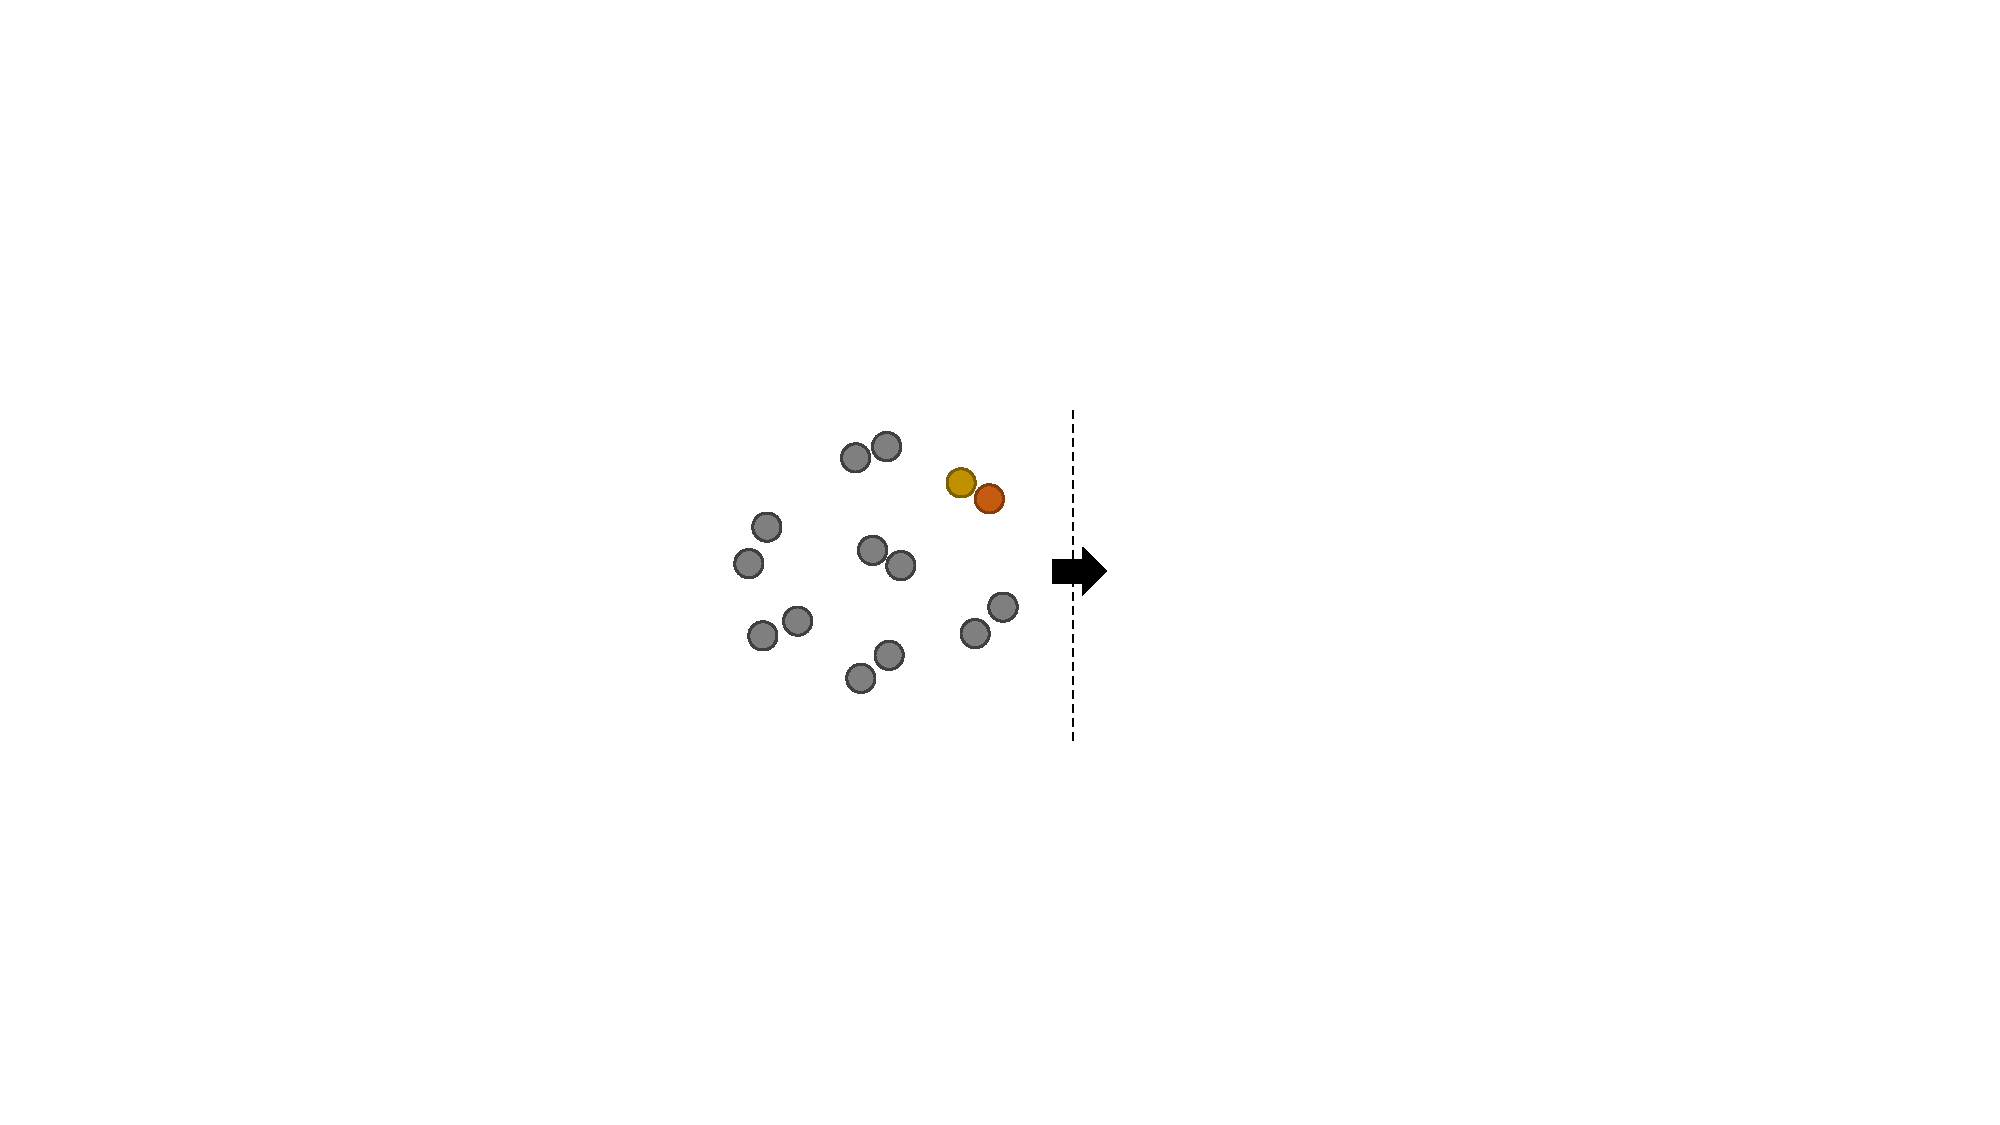
\includegraphics[width=\textwidth]{Img/fig_5_cat_b.pdf}
      \caption{}
      \label{fig:5_cat_b}
    %\end{minipage}
    \end{subfigure}
    % line break
    \begin{subfigure}[b]{0.38\textwidth} % default 0.32\textwidth
    %\begin{minipage}[t]{0.33\linewidth}
      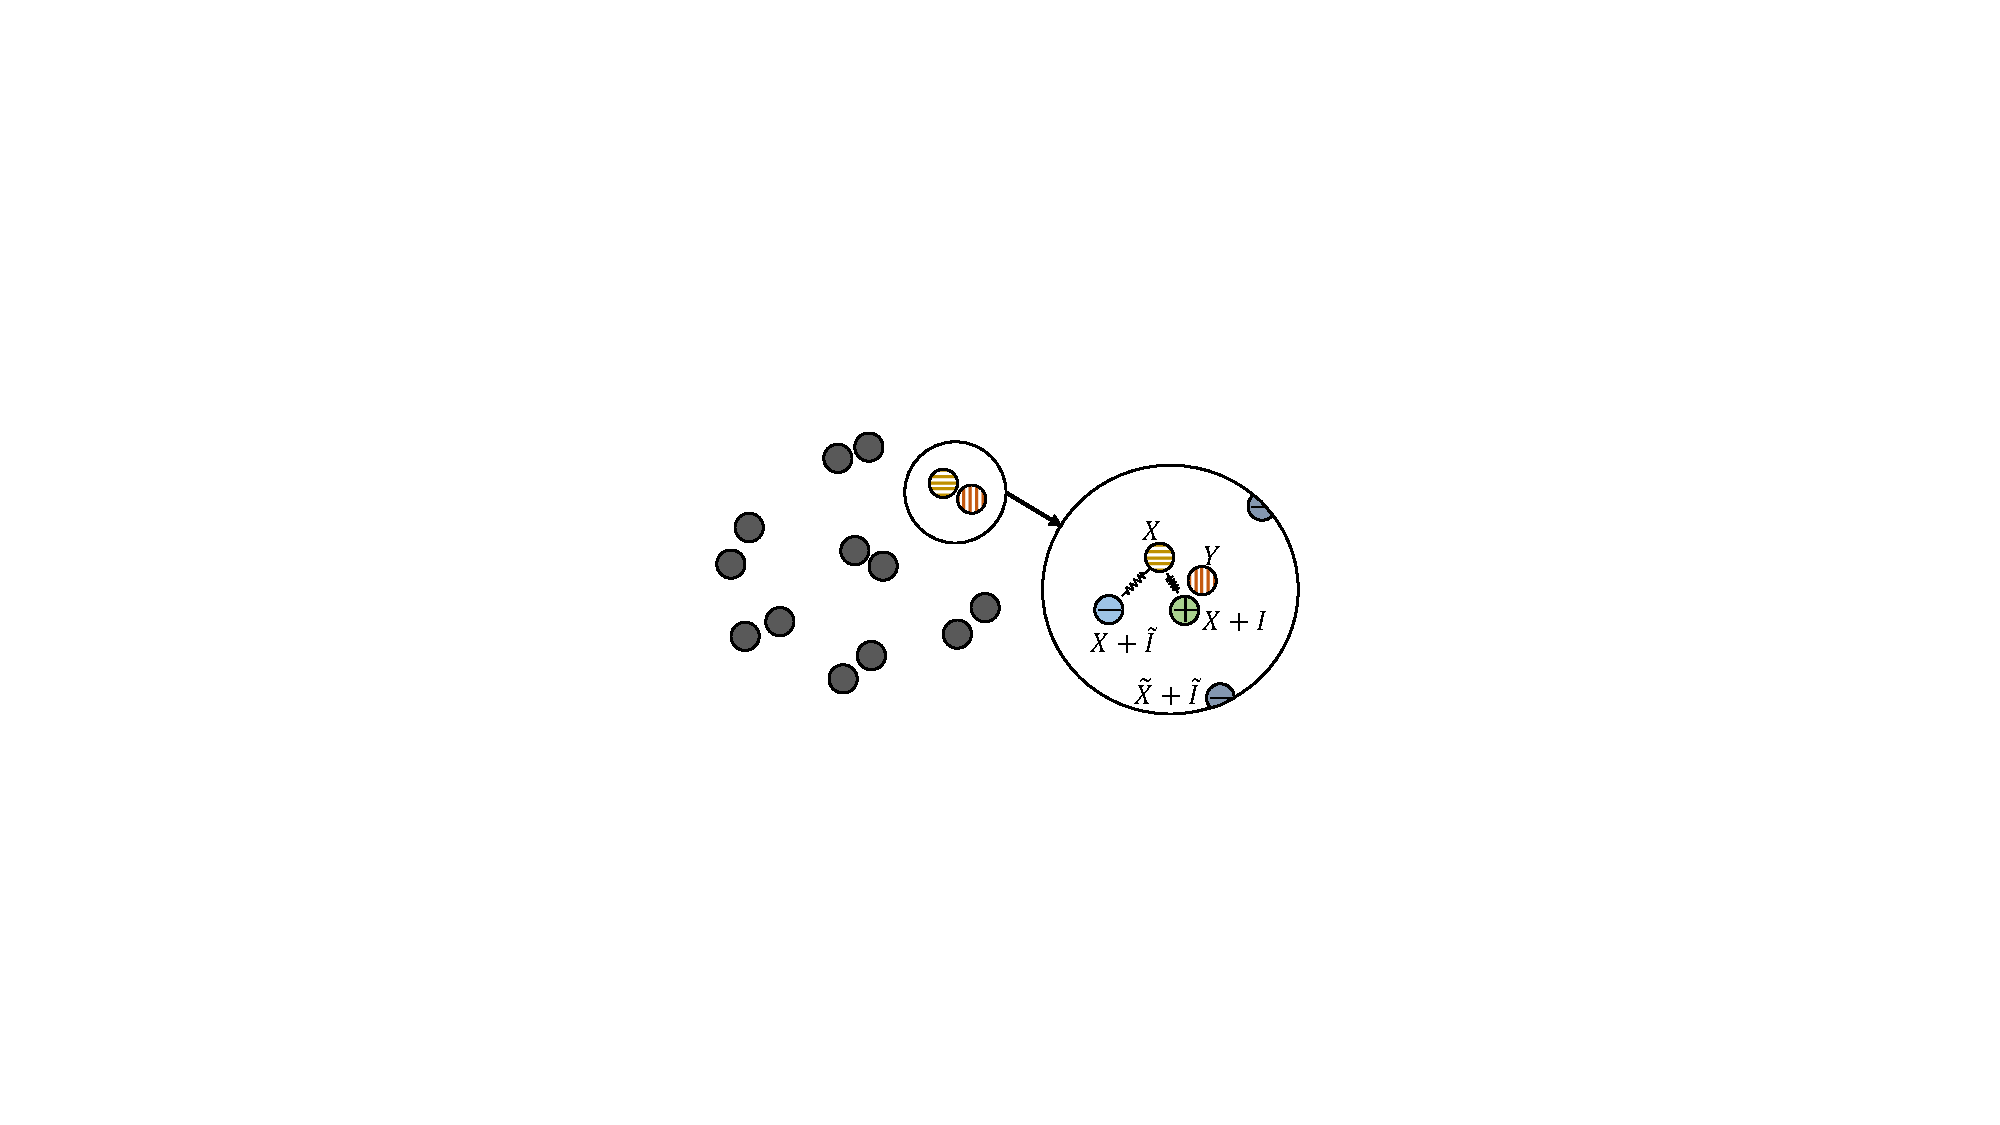
\includegraphics[width=\textwidth]{Img/fig_5_cat_c.pdf}
      \caption{}
      \label{fig:5_cat_c}
    %\end{minipage}
    \end{subfigure}%
    \bicaption{对比对抗训练方法原理示意图}{Schematic diagram of the principle of contrastive training method}
    \label{fig:5_cat}
\end{figure}

{\sffamily (1)对比学习}

对比学习方法能够在语义表示空间中拉近相似的样本,推离不相关的样本。在融合图片信息的神经机器翻译中,将目标译文$Y$作为锚点,将编码端的输入$X+I$作为正样本。在$X$与$Y$的双语统一表示空间中,对比学习方法能够拉近$X+I$与$Y$之间的距离,并将其它的所有样本视为负样本,拉开与$X+I$和$Y$之间的距离。图\ref{fig:5_cat}中每个圆代表文本语义表示空间的一个点,其中图\ref{fig:5_cat}(a)和图\ref{fig:5_cat}(b)展示了对比学习将表示空间的样本分簇归类的能力,图\ref{fig:5_cat}(b)中的每个簇可视为一个双语平行句对。常规的对比学习(contrastive learning,CL)损失函数为:
\begin{equation}
    \mathcal{L}_{CL}(\theta, \psi)=-\log\ \frac{e^{\mathrm{cos}(\mathrm{A}(Y),\mathrm{A}(X+V))/\tau}}{\sum_{Z\in N}e^{\mathrm{cos}(\mathrm{A}(Y),\mathrm{A}(Z))/\tau}}
    \label{eq:5_contrastive_learning}
\end{equation}

其中$\mathrm{cos}(\cdot,\cdot)$为余弦相似度函数,用于计算两个表示向量的语义相似度;$\tau$为温度,控制区分正负样本的能力;$\mathrm{A}(\cdot)$代表平均池化,正如图\ref{fig:5_model}所示,对比损失的输入是文本表示经平均池化后的结果;$N$代表着负样本集。

$\mathcal{L}_{CL}$与$\mathcal{L}_{CE}$之间共享编码器和跨模态嵌入层的参数,因此本章所采用的对比学习只针对编码器进行参数优化,从而使编码器具备利用图片信息辅助句子编码的功能。

{\sffamily (2)对抗训练}

尽管采用对比学习方法能够拉近相似样本$X+I$与$Y$之间的语义关系,并增加与其它样本之间的距离,但是该过程并不能保证翻译模型利用到了图片$I$中的信息。这是因为在机器翻译任务所使用的数据中,多数的原文$X$与译文$Y$都保持着良好的对齐关系。并且对于翻译任务所需要的信息而言,大部分$X$与$X+I$所能提供的语义信息的差距也很小。当模型对视觉信息不敏感时,即便输入的是$X+I$,模型仅通过输入中的文本信息$X$就可以得到相对可用的结果,且该过程相比于提取图片中的跨模态信息是更容易的。这一点对于融合跨模态信息的神经机器翻译和对比学习拉近语义关系均是通用的。

为了让模型具备融合视觉信息的能力,首先需要使模型具备更细粒度的语义聚类的能力。如图\ref{fig:5_cat}(c)所示,为了让模型区别出$X$与$X+I$之间的差别,就需要在原对比学习的基础上增加其它可对比的信息。因此,本章针对负样本集$N$进行了相应的改进:
\begin{equation}
    N=N_{AS}\cup B_{\setminus X}
    \label{eq:5_negative_sample_set}
\end{equation}
\begin{equation}
    N_{AS}=\{X+\tilde{I},\tilde{X}+\tilde{I}\}
    \label{eq:5_adversarial_sample_set}
\end{equation}
其中$\tilde{I}$为随机图片;$\tilde{X}$为退化句子,其内部与视觉目标相对应的词被替换为特殊字符“<mask>”;$B_{\setminus X}$代表同批数据中除$X$外的其它样本;$N_{AS}$为对抗样本集。

在对抗样本集$N_{AS}$中,$X+\tilde{I}$有着与$X$以及$X+I$更近的语义关系,$\tilde{X}+\tilde{I}$次之。但$N_{AS}$是负样本集的子集,此时带有源语言信息的$X$同时出现在正样本集和负样本集中。对比学习方法想要区分开正负样本就需要从输入文本以外的图片中获取差异化的信息。上一节中提到,解码器仅依靠“文本模态”的隐层表示生成译文。为了给解码器提供更好的编码结果,在对比学习阶段也仅采用“文本模态”的隐层表示作为输入。这意味着当模型的输入为$X+I$时,对比学习为了获取到图片带来的差异化信息,需要迫使编码器将图片$I$中的信息融合到文本$X$的隐层表示中。因此,为了使神经机器翻译利用到视觉信息,采用对比对抗训练方法时一方面需要将对抗样本加入到负样本集中,另一方面需要保证视觉信息融合到文本的隐层表示中。

{\sffamily (3)双向翻译训练}

在公式(\ref{eq:5_contrastive_learning})中可以观察到,计算对比损失时,译文$Y$作为锚点同样需要参与计算过程。这表示Transformer的编码器不仅负责源语言端的文本加图片的编码,还要支持目标端语言的纯文本编码。然而,在一个常规的单向翻译任务中,仅源端语言在编码器中得到了优化。在本章所提方法中,源语言的编码会通过翻译任务的目标函数$\mathcal{L}_{CE}$联合对比学习的目标函数$\mathcal{L}_{CL}$得到优化。而目标语言在编码器中仅能得到对比学习的目标函数的优化。这种不平衡的优化方式可能会对CAT方法带来负面效果。因此,需要采用双向翻译训练(bi-directional translation training,BDTT)解决这个问题。在训练的过程中,模型将用于两个翻译方向的训练。其中源语言到目标语言的训练是在编码端融合图片信息的翻译训练,目标语言到源语言的训练是纯文本的训练过程。需要注意的是,BDTT方法影响的是目标语言的编码质量。没有BDTT的情况下,CAT方法依旧可以工作,只不过$\mathcal{L}_{CL}$损失函数需要从模型的初始随机状态优化目标语言的编码。

\subsection{与神经机器翻译结合}
\label{sec:5_combine_with_nmt}

为了得到联合损失函数,本文联合公式(\ref{eq:5_cross_entropy})与公式(\ref{eq:5_contrastive_learning})得到:
\begin{equation}
    \mathcal{L}=\mathcal{L}_{CE} + \lambda|X|\mathcal{L}_{CL}
    \label{eq:5_combine_with_nmt}
\end{equation}
其中$\lambda$是平衡交叉熵损失和对比损失的超参数。$|X|$代表句子$X$的句长。因为$\mathcal{L}_{CL}$中需要对隐层单元经过平均池化层,所以$\mathcal{L}_{CL}$需要乘以句长$|X|$从而与$\mathcal{L}_{CE}$同为句子级别的计算结果。